\chapter{Bollard Pull}
\label{app:bollpull}

\section{Purpose}
The purpose of this measurement journal is to test if the force, which is generated from the vessel, is linear with the control input to the thrusters or if there should be a mapping between these.

\section{Theory}
If the linear stepped input to the thrusters ends out in a linear output of the vessel it can be approximated that the translation from input to output is linear. This makes some of the controlling of the vessel less complicated due to the non existing non linear mapping from input to output. If a mapping is needed this needs to be taken care of in the control of the vessel, which needs to be compensated at least in the simulations of the vessel. This makes it possible to take it into account in the plant model of the vessel but might be neglected in the control model.

\section{Tools}
\begin{table}[htbp]
\centering
\begin{tabular}{ccc}
	\toprule
  Tool \\
  \midrule
  Test vessel \\
  Dynamometer \\
  Rod to apply on the vessel \\
  	\bottomrule
\end{tabular}
\caption{Tools needed to test the forces generated by the vessel.}
\label{tab:bollpulltool}
\end{table}

\section{Method}
The first tests, utilizing the thrusters forward, was performed by applying a rod symmetric at the stern of the vessel. The rod was extended such that it was possible to measure the force generated by the vessel from the bay, while the vessel was in the middle of the lake. This is done to make the reflecting waves as little as possible. The same procedure are used when testing the vessel while thrusting backwards. The test setup can be seen on figure .

\begin{figure}[htbp]
	\centering
	\includesvg[width=0.6\textwidth]{bollpullsetup}
	\caption{Setup while testing bollard pull, forward and backward motion.}
	\label{fig:bollpullsetup}
\end{figure}


\section{Results}
\begin{figure}[htbp]
	\centering
	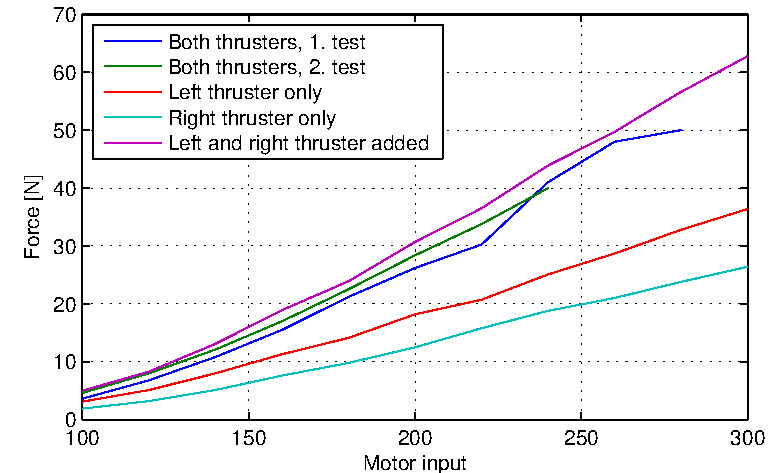
\includegraphics[width=0.6\textwidth]{plot/forwardthrust}
	\caption{Forward motion tests.}
	\label{fig:bollpullforward}
\end{figure}

\begin{figure}[htbp]
	\centering
	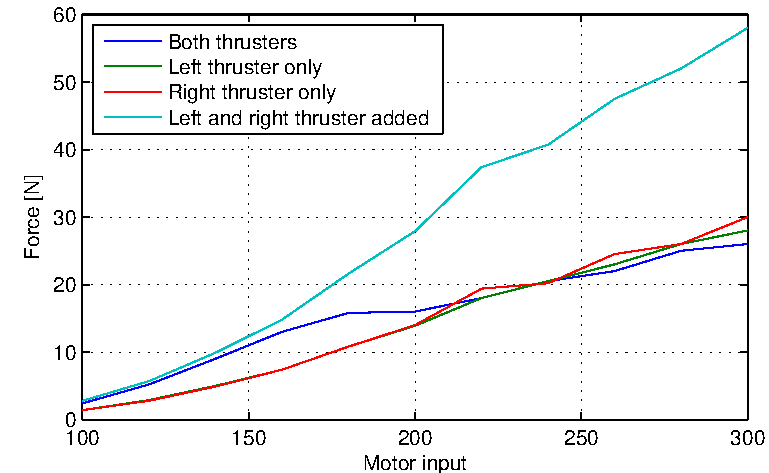
\includegraphics[width=0.6\textwidth]{plot/backthrust}
	\caption{Backward motion tests.}
	\label{fig:bollpullbackward}
\end{figure}

\section{Discussion and conclusion}
In both the forward and backward test comes one issue into account. When the vessel is applied with motor inputs above 200 will the ventilation at the propellers become too significant. The stern of the vessel will rises so much that
